\documentclass[
BCOR0.7cm,							% Bindekorrektur, bspw. 1 cm
]
{scrbook}

\newif\ifpdf
\ifx\pdfoutput\undefined
	\pdffalse              	%normales LaTeX wird ausgef�hrt
\else
	\pdfoutput=1           
	\pdftrue               	%pdfLaTeX wird ausgef�hrt
\fi

\ifpdf %%Einbindung von Grafiken mittels \includegraphics{datei}
	\usepackage[pdftex]{graphicx} %%Grafiken in pdfLaTeX
\else
	\usepackage[dvips]{graphicx} %%Grafiken und normales LaTeX
\fi

\ifpdf
	\pdfinfo
	{
    /Author (Manfred Kindl)                                
    /Title (Abgabetool)     
    /Subject (Benutzerhandbuch Abgabetool)                                    
    /Keywords (Abgabe Abgabetool FH-Complete Technikum-Wien)
	}
\else			
\fi

\usepackage{listings} \lstset{numbers=left, numberstyle=\tiny, numbersep=5pt}
\lstset{language=tex} 

\usepackage[pdftex,colorlinks=true,urlcolor=blue,linkcolor=blue]{hyperref}
\usepackage[ngerman]{babel}		
\usepackage[T1]{fontenc}
\usepackage[latin9]{inputenc}
\usepackage{makeidx}
\usepackage{float}
\usepackage[small,bf]{caption}
\usepackage{fancyhdr}
\usepackage{amssymb,amsmath}
\makeindex

\graphicspath{{../../images/}}

\setlength{\tolerance}{2000}
\setlength{\parindent}{0pt}
\setlength{\parskip}{1ex plus 0.5ex minus 0.2ex}
\addtolength{\textheight}{2cm}
\addtolength{\headheight}{2pt}
\setlength{\captionmargin}{20pt}
\floatstyle{plain}
\floatname{example}{Example}

\newfloat{example}{hbtp}{loe}[chapter]
\floatplacement{figure}{hbtp}
\floatplacement{table}{htbp}

\newcommand{\dollar}{\char36}

\newenvironment{info}[1]
{
    \hspace{-10mm}
    \fbox
    {
        \begin{minipage}{1cm}
        
\includegraphics[width=1cm]{icon_info}
        \end{minipage}
        \begin{minipage}{14.5cm}
        #1
        \end{minipage}
    }
}

\newenvironment{achtung}[1]{
    \hspace{-10mm}
    \fbox{
        \begin{minipage}{1cm}
        
\includegraphics[width=1cm]{icon_achtung}
        \end{minipage}
        \begin{minipage}{14.5cm}
        #1
        \end{minipage}
    }
}

\newenvironment{halt}[1]{
    \hspace{-10mm}
    \fbox{
        \begin{minipage}{1cm}
        
\includegraphics[width=1cm]{icon_halt}
        \end{minipage}
        \begin{minipage}{14.5cm}
        #1
        \end{minipage}
    }
}

\newenvironment{idee}[1]{
    \hspace{-10mm}
    \fbox{
        \begin{minipage}{1cm}
        
\includegraphics[width=1cm]{icon_idee}
        \end{minipage}
        \begin{minipage}{14.5cm}
        #1
        \end{minipage}
    }
}


\setlength{\unitlength}{1mm}

\newenvironment{markier}[5]
{    
    \thicklines \put(#2,#3){\vector(#4,#5){5}} \thinlines
    \put(#2,#3){\circle*{5}}
    \put(#2,#3){\textcolor{black}{\circle{5}}\makebox(-10,0){\textcolor{white}{#1}}}
}


\hyphenation{gleich-zeitig para-meter}


\begin{document}

\ifpdf
	\DeclareGraphicsExtensions{.pdf,.jpg,.png}
\else
	\DeclareGraphicsExtensions{.eps}
\fi

\pagestyle{fancyplain}
% Titelseite einbinden

%
% Titelseite, Abstrakt, Danksagung und Inhaltsverzeichnis
%
%% eigene Titelseitengestaltung %%%%%%%%%%%%%%%%%%%%%%%%%%%%%%%%%%%%%%%    

\begin{titlepage}
\begin{center}
\vspace*{30mm} \Huge Abgabetool\\
\vspace*{10mm}
%\large \textsc{Untertitel}

\vfill 
\includegraphics[width=136mm]{cis}\\
\vspace*{20mm}
\textsc{\LARGE{Handbuch f�r Lektorinnen und Lektoren}\\
\vspace*{5mm}
\large{Stand \today}}

	
\vfill \small{FH Technikum Wien}\\

\end{center}
\end{titlepage}



\tableofcontents			% Inhaltsverzeichnis

\frontmatter					% Vorspann (z.B. r�mische Seitenzahlen)

\chapter{Einleitung}
\label{Kapitel Einleitung}

Dieses Handbuch erl�utert die Benutzung und Funktion der Bachelor- und Diplomarbeitsabgabe (kurz Abgabetool) auf der CIS-Seite der FH Technikum Wien.

Das Abgabetool dient zur Interaktion zwischen LektorInnen und Studierenden rund um die Abgabe von Projektarbeiten (Bakk- bzw Diplomarbeiten).
Studierende haben die M�glichkeit, zu definierten Terminen Dokumente hochzuladen.\\
Lektoren k�nnen Abgabetermine (f�r einzelne oder mehrere Studierende) und Abgabefristen definieren und hochgeladene Dokumente betrachten und bewerten.



\mainmatter						% Hauptteil

%% Kapitel Anfang %%%%%%%%%%%%%%%%%%%%%%%%%%%%%%%%%%%%%%%%%%%%%%%%%


\chapter{Abgabetool f�r LektorInnen}
\label{Kapitel Aufruf}
Der Aufruf der LektorInnenoberfl�che erfolgt �ber cis.technikum-wien.at/Mein CIS/Bachelor- und Diplomarbeitsabgabe.

\section{�bersichtsliste der Betreuungen}
In der �bersichtsliste (siehe Abbildung \ref{abgabetool_uebersichtsliste}) finden sich alle Betreuungen von Bachelor- und Diplomarbeiten (im FAS unter Projektarbeit als �berbegriff zusammengefasst, daher der Name Projektarbeitsabgabe), deren Autorin oder Autor noch aktiv sind.

\begin {figure}
	\centering
	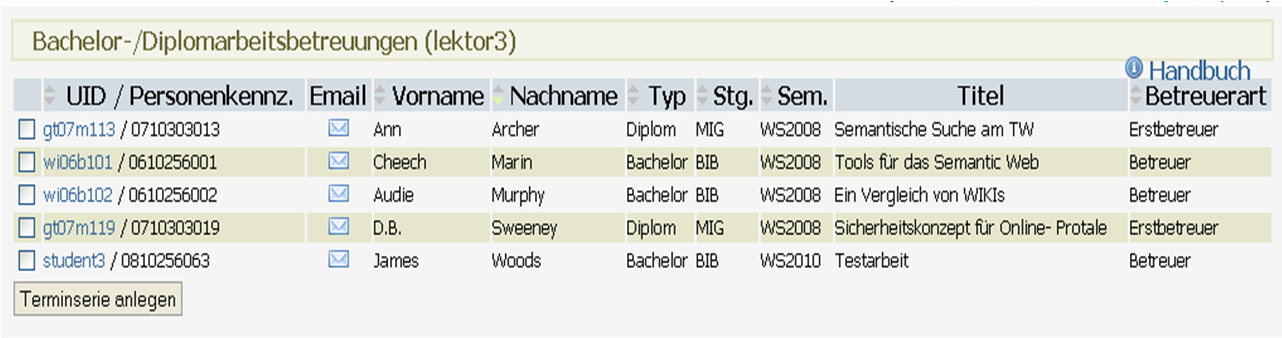
\includegraphics[width=1.0\textwidth]{abgabetool_uebersichtsliste}
	\caption{�bersichtsliste der betreuten Arbeiten}
	\label{abgabetool_uebersichtsliste}
\end {figure}

\subsection{Aufrufen der Termin�bersicht}
Durch Anklicken der UID der Studentin/des Studenten in der zweiten Spalte der �bersichtsliste werden die Termindetails im unteren Teil der Seite angezeigt (Siehe Abbildung \ref{abgabetool_terminverwaltung}).

\subsection{E-Mail an die Studentin/den Studenten}
Durch Anklicken des Briefsymbols in der dritten Spalte wird der E-Mailclient ge�ffnet und die Empf�nger- und Absenderadresse sowie \textit{Bachelorarbeitsbetreuung} bzw. \textit{Diplomarbeitsbetreuung} als Betreff werden vorausgef�llt.

\subsection{Termin f�r mehrere Studentinnen und Studenten ansetzen}
Es gibt auch die M�glichkeit, f�r mehrere Studentinnen und Studenten einen Termin zu setzen. Dazu m�ssen zuerst die betreffenden Zeilen durch Anklicken der Checkbox in der ersten Spalte markiert werden. Danach �ffnet ein Klick auf den Button \textit{Terminserie anlegen} eine Eingabemaske im unteren Teil des Browserfensters. Hier wird dann der Termin eingegeben und durch Dr�cken der Taste \textit{speichern} der Termin f�r alle zuvor markierten Betreuungen gespeichert.

\subsection{Aufruf der Anleitung}
Rechts neben der �berschrift \textit{Bachelor- /Diplomarbeitsbetreuungen} befindet sich ein blauer Icon mit einem weissen i. Durch einfaches Klicken darauf kann diese Anleitung als pdf-Datei aufgerufen werden.

\section{Termin�bersicht}

\begin {figure}
	\centering
	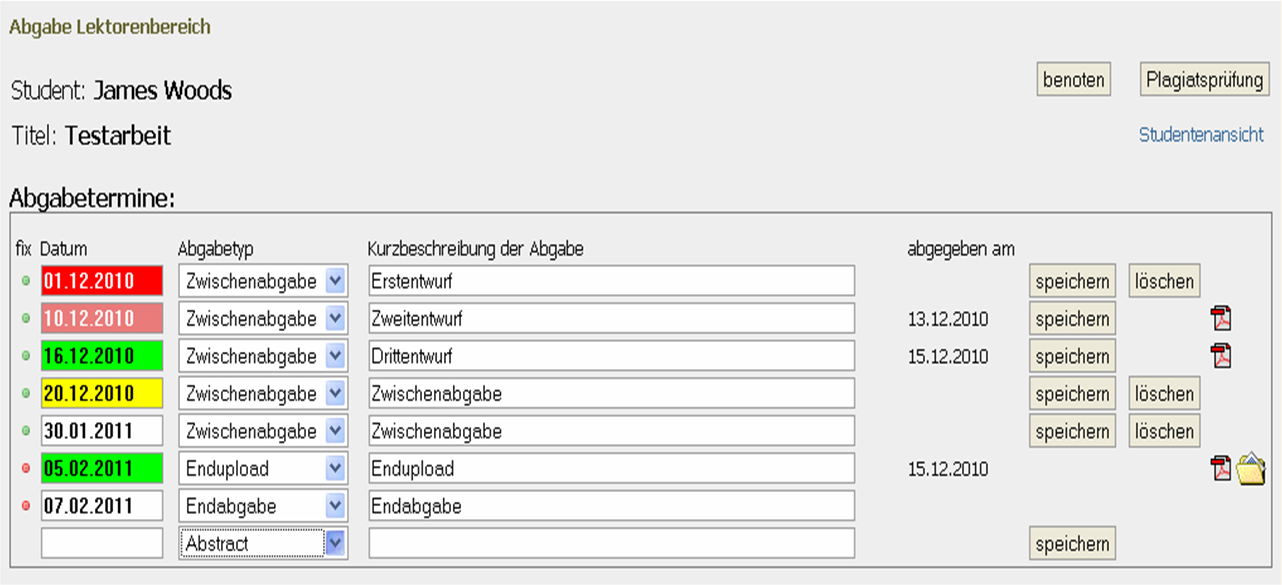
\includegraphics[width=1.0\textwidth]{abgabetool_terminverwaltung}
	\caption{Verwaltung und �bersicht der Termine}
	\label{abgabetool_terminverwaltung}
\end {figure}

\subsection{Termineingabe und -bearbeitung}

\begin{itemize}
	\item Termineingabe: Die unterste Zeile der Liste ist bis auf das Auswahlfeld \textit{Abgabetyp} leer und f�r die Eingabe eines neuen Termins vorgesehen. Geben Sie ein Datum ein, w�hlen Sie den Abgabetyp aus und geben Sie eine kurze Beschreibung der Abgabe ein. Abschlie�end wird mit einem Klick auf den Button \textit{speichern} der Termin eingetragen.
	\item Termin�nderung: Termineintr�ge k�nnen ge�ndert werden, indem Sie die Daten der betreffenden Zeile �ndern und anschlie�end \textit{speichern} dr�cken.
	\item Termin l�schen: Termin k�nnen durch Klicken auf die Taste \textit{l�schen} gel�scht werden. Ist bereits eine Abgabe erfolgt, kann ein Termin nicht mehr gel�scht werden.
	
	\info{�ber alle drei Aktionen wird die Studentin/der Student per Mail informiert}
	\item Die Assistenz kann fixe Termine vergeben, erkennbar an dem roten Bullet unter \textit{fix}. Liegt ein Termin in der Vergangenheit, kann die Studentin/der Student zu diesem nichts mehr hochladen. Soll dennoch etwas hochgeladen werden, mu� die Studentin/der Student bei der Studiengangsassistenz um eine Korrektur des Termins ansuchen.
	
	\info{Es k�nnen nur selbst angelegte Termine ge�ndert und gel�scht werden}
\end{itemize}

\subsection{Farbcode}

\begin{itemize}
	\item wei�:	"normaler" Termin
	\item gelb:	Termin innerhalb der n�chsten 12 Tage
	\item rot:	Termin �berschritten
	\item gr�n:	Abgabe erfolgt
	\item hellrot: Abgabe nach Termin 
\end{itemize}

\subsection{Download der Abgabe und Ansicht der Zusatzdaten}
Durch Klicken auf das Symbol 
\includegraphics{icon_pdf} wird ein Dialogfenster zum Speichern oder Betrachten der Abgabe dieses Termins ge�ffnet.
Bei der Endabgabe m�ssen von der Studentin/dem Studenten zus�tzlich Daten f�r die Publikationsdatenbank eingegeben werden. Diese sollten mittels dem Symbol 
\includegraphics{icon_ordner_endabgabe} vor der Benotung �berpr�ft werden.

\subsection{Benotung}
Rechts oben auf der Temin�bersicht befindet sich der Button \textit{benoten}, mit dem das Formular zur Benotung der Bachelor- bzw. Diplomarbeit aufgerufen werden kann. Die bereits verf�gbaren Daten wie die Daten der Studentin/des Studenten, Titel der Arbeit, Name der Begutachterin/des Begutachters sind bereits vorausgef�llt. Eingetragen m�ssen die verbalen Beschreibungen der Teilbenotungen und die Punkte der Teilbereiche. Aus den Punkten werden nach dem am Formular aufgef�hrten Schl�ssel die Noten sofort mit der Eingabe berechnet. 

Das Formular wird abschlie�end ausgedruckt und unterschrieben bei der Studiengangsassistenz abgegeben.

\subsection{Link zur Plagiatspr�fung}
Neben dem Button f�r das Benotungsformular befindet sich der Aufruf der Internetseite zur Plagiatspr�fung. Dort kann die abgegebene Arbeit hochgeladen werden.

\subsection{Studentenansicht}
Unterhalb des Links zur Plagiatspr�fung wird ein Link f�r die Studentenansicht angezeigt.
Hier wird die Abgabe aus Studentensicht angezeigt. Sie k�nnen von hier aus auch Arbeiten f�r die Studenten hochladen.

\subsection{Termin�bersicht f�r alle Termine}
Unterhalb der Liste der Studierenden gibt es die M�glichkeit, eine Liste mit allen Abgabeterminen der betreuten Studierenden zu erstellen. In dieser Liste werden alle Termine angezeigt die noch in der Zukunft liegen.

\subsection{Alte Arbeiten anzeigen}
Sie k�nnen sich die Termine und Arbeiten der abgeschlossenen Betreuungen einblenden, indem Sie unterhalb der Liste der Studierenden auf den Link "alle betreuten Arbeiten anzeigen" klicken. Es werden dann in der Liste, zus�tzlich zu den normalen Betreuungen, auch die Betreuungen angezeigt die bereits benotet wurden.


%% Kapitel Ende   %%%%%%%%%%%%%%%%%%%%%%%%%%%%%%%%%%%%%%%%%%%%%%%%%
\appendix							% Beginn des Anhangs
%\chapter{Schluss}
%\listoftables				% Tabellenverzeichnis
%\listoffigures				% Abbildungsverzeichnis

\end{document}
